\subsection{Definition}
The Lagrangian relaxation is a procedure that find a lower bounds. This lower bounds will allow to have better performances on the branch and bounds of the problem starting with an initially good lower-bounds.
We first relax the problem with the Lagrangian relaxation we then optimize the $\lambda$ with a sub-gradient algorithm and we get the optimal $\lambda$ and thus the optimal solution of the relaxed problem which is a good lower bounds.

\subsection{Example}
In order to represents the concepts discussed in this section, we will need an example. Lets take the Constrained Shortest Path problem.

\centerline{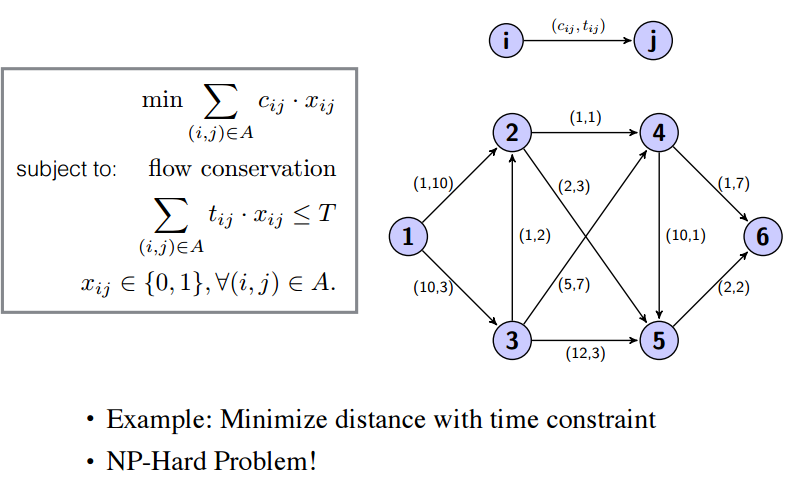
\includegraphics[scale=0.7]{lagrangeexample.png}}

\subsection{Relaxation}
If we remove the resource constraint, the problem is pretty easy. It is a simple shortest path problem that can be easily resolved with Dijkstra. What the Lagrangian relaxation does is removing the constraint and adding a new part in our minimization part.

\centerline{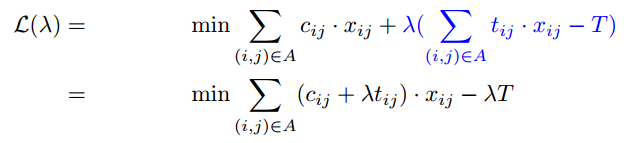
\includegraphics[scale=0.7]{lagrange1.png}}

We now have a simple shortest path problem with edges that weight a mixed value of time and distance for a given value of $\lambda$. Using this minimization with different $\lambda$ will return different solutions. Some of them won't be feasibly and will violate the time constraint. If you are lucky one of the solution will be the optimal one. (hint : try $\lambda = 2$)

\subsection{Lagrangian dual}
Now our objective will be to find the best $\lambda$ in order to have the best feasible solution (the best we can have with Lagrangian, not necessarily the best of the actual problem, this algorithm is only used to have a lower bound). We have our Lagrangian dual : 

\centerline{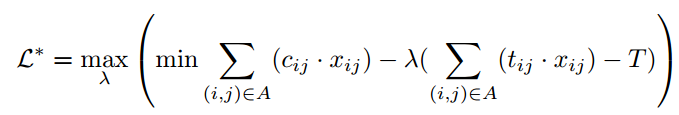
\includegraphics[scale=0.7]{lagrangiandual.png}}

\subsection{Sub-gradient algorithm}

\subsubsection{Idea}

The sub-gradient algorithm will allow us to find the best $\lambda$. The idea is simple. Take an initial $\lambda$ and calculate the solution (Dijkstra resolution). Then we check if we are on a increasing edge (violation of the constraint) or a decreasing edge (constraint is respected). Depending of that we will respectively move to the right or to the left.

\centerline{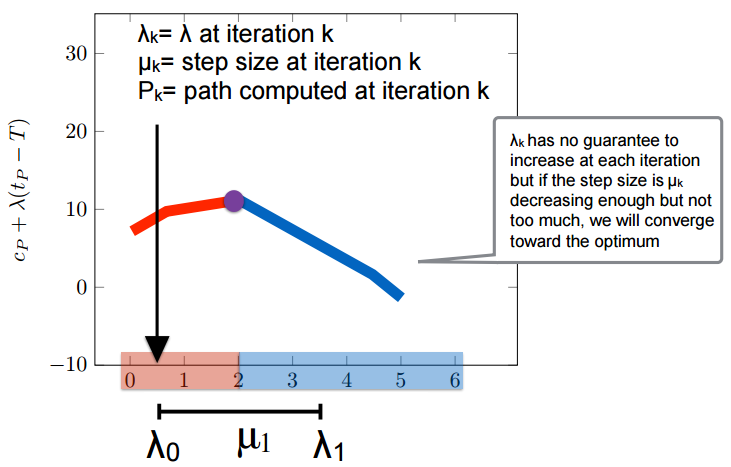
\includegraphics[scale=0.7]{lagrangiangraph.png}}

In order for the algorithm to converge we must reduce the size of the step at each iteration. It is guaranteed to converge if $\mu_{k} \rightarrow 0$ and $\sum^{k}_{j=1} \mu_{k} \rightarrow \infty$.
On the other hand the Lagrangian lower bounds has no guaranteed to increase at each step.

\subsubsection{Pseudo-code}

\centerline{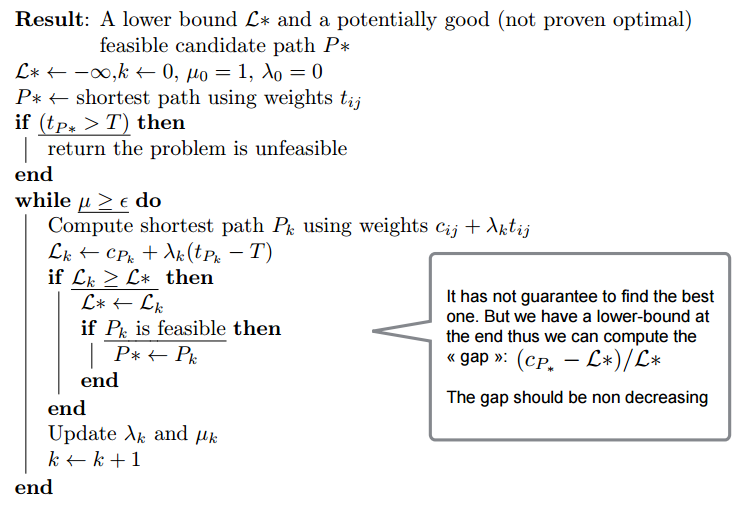
\includegraphics[scale=0.7]{lagrangepseudocode.png}}

\subsection{Performances}

The Lagrangian relaxation is as good as the linear relaxation. But the advantage of the Lagrangian one is that it will return feasible solution during the process.

Typically the lower bounds will evolve along a curve that converge after x steps.

\centerline{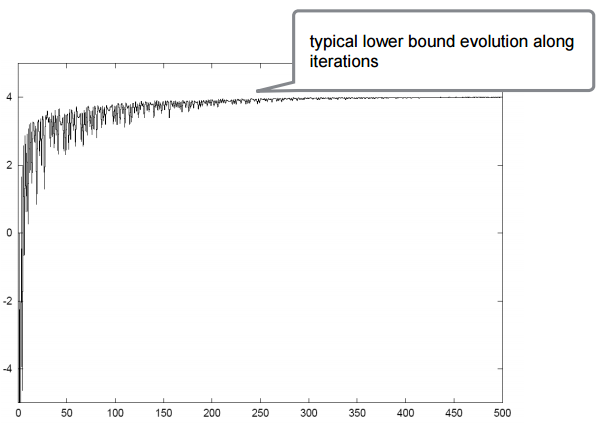
\includegraphics[scale=0.8]{lagrangeconverge.png}}